% Chapter Template

\chapter{Results of flow field noise analysis} % Main chapter title

\label{results} % Change X to a consecutive number; for referencing this chapter elsewhere, use \ref{ChapterX}

\lhead{\emph{Results of flow field noise analysis}} % Change X to a consecutive number; this is for the header on each page - perhaps a shortened title

%----------------------------------------------------------------------------------------
%	SECTION
%----------------------------------------------------------------------------------------

\section{Transition from flow-field to sound signal data}

The performed DDES analysis delivered a set of files for further postprocessing. Values of static pressure, velocity magnitude, vorticity magnitude, static density and static temperature were gathered from designated boundaries and internal surfaces representing the design streamline cones. The dataset consists of 50150 files for each of the 13 internal surfaces and 5 blade boundaries, resulting in over 5.5 TB of data.

This set was postprocessed to obtain the sound pressure, sound intensity and their respective decibel values for each time step. The mathematical formulas for obtaining these values are provided in chapter \ref{approach} and the \texttt{Python 3.5x} implementation of which is presented in appendix \ref{codedirect}. The postprocessing of flow field data to sound data was performed on the same HPC infrastructure as the DDES analysis, due to the file accessibility. Postprocessed dataset was saved in a folder structure resembling the source files. The dataset consists of 902 700 files and another 5.5TB of data in form of comma separated values.

%-----------------------------------
%	SECTION
%-----------------------------------
\section{RMS results} \label{rms}

%-----------------------------------
%	SUBSECTION
%-----------------------------------
\subsection{Results postprocessing} \label{rms_res_prep}
The time specific sound pressure values were further processed to obtain the Root Mean Square values of sound pressure and sound intensity from internal markers and blade surfaces. Due to large number of figures, the scatter plots of the aforementioned values are provided in the Appendix \ref{rms_results}n in figures \ref{blade-rms-spl} thru \ref{int-tip-rms-sildb}. Providing data for both pressure and intensity values and their decibel levels is redundant, yet both plots are shown for clarity and direct comparison of given values. 

Internal boundary plots provide information on maximum and minimum values of SPL and SPLdB presented on the plot. As the minimum sound intensity (SIL) is equal 0 and the SILdB values for corresponding points approach negative infinity. Such values were overridden to show 0 SILdB on the plot.    For this reason minimum value coordinates are omitted in the plot description 

Blade surface plot is composed by plotting five datasets on one canvas and manipulating the sign of the canvas x-axis to mimic various view projections. Tool used to generate the scatter plots for blade surface overlaps the datapoints that share the same canvas x and canvas y coordinates, therefore the plotting order is always "back-to-front", so that the surface closest to the viewer is plotted atop the canvas.

Sound pressure and intensity plots are scaled with a normalized logarithmic colorbar with common scale across all of the internal surface and blade surface plots. For sound pressure, the maximum obtained value is $13917.395 [Pa]$, so the maximum value of the colorbar is liberally rounded up to $15000 [Pa]$. Minimum value for SPL is in range of $10 [Pa]$, so the lower bar limit is set to zero. As for the Decibel values the lowest obtained value is around $116 dB$, largest - around $177 dB$. The colorbar scale is therefore set to 100 - 180 dB range with linear scale. The same approach was used for maximum values of sound intensity. For sound intensity itself, the colorbar was limited from $0 W/m^2$ to $1.2 \cdot 10^6 [W/m^2]$ and normalized to logarithmic scale. For SILdB plot, the bar range is limited to $0 dB$ to $180 dB$ range with linear scale. %More details on RMS values are presented in section \ref{numbers}. 

Plots are created by projecting points from 3D surface onto a 2D plane of the plot, therefore some shape aberrations may occur. Color of the point is normalized as described above. The axes names correspond to the global coordinate system axes. Length unit for all plots is meter.

%-----------------------------------
%	SUBSECTION
%-----------------------------------
\subsection{Qualitative analysis} \label{rms_res_qual}
Averaged sound pressure and sound intensity plots provide some information on the character of the acoustic phenomena modelled in a stationary reference frame for given test compressor.

The sound pressure fluctuations that translate to high SPLdB values occur in regions where flow is turbulent. For internal controll surfaces, where flow is globally subsonic (int-01, int-02, int-03 -- figures \ref{int-01-rms-sil} thru \ref{int-03-rms-sildb}), the sources of the aerodynamically induced noise correspond to the regions on flow separation on the suction (upper on the plots). This is especially visible in the wake of the blade. Figures \ref{blade-rms-spl} and \ref{blade-rms-spldb} provide the view of the blade's suction surface. A separation of the flow at leading-edge-to-hub transition leading to a very characteristic secondary flow and corner stall separation (separated flow on the suction surface near the trailing-edge-to-hub transition). The largest pressure fluctuations were noted on the trailing edge and trailing-edge-to-tip transition, which is visible on both blade surface plots and internal surfaces plots.

Internal surface contour plots show, that the source of sound pressure is the supersonic-to-subsonic transition occurring on the shockwave. The effect of shock induced flow separation is becoming visible on internal surface plots for surfaces int-04 and int-05 (figures \ref{int-04-rms-spl} thru \ref{int-05-rms-sildb}), with full visibility of described phenomena on surfaces int-06 thru int-12 (figures \ref{int-06-rms-spl} thru \ref{int-12-rms-sildb}). Plot for surface adjacent to the blade tip (surface int-tip, figures \ref{int-tip-rms-spl} thru \ref{int-tip-rms-sildb}) show the effect of "tip-leakage" phenomena when high pressure flow at the pressure side of the compressor creeps to the low pressure suction side thru the tip gap (Fig. \ref{tip_stream}). 

\begin{figure}[h!]
\centering % bo \centering nie wstawia dodatkowego odstępu
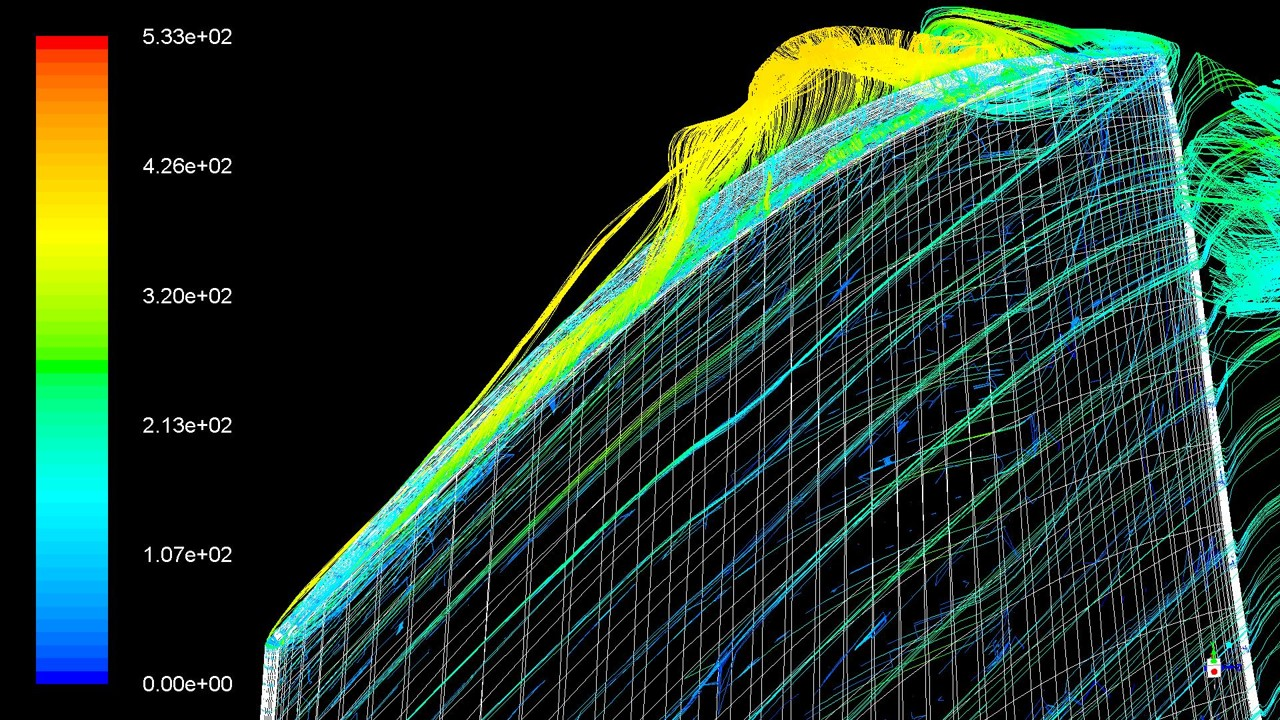
\includegraphics[width=0.85\textwidth]{Pictures/tip_stream.jpg}
\caption{Tip gap streamlines. Velocity in [m/s]}
\label{tip_stream}
\end{figure}

Presented contour plots show a rather significant noise level in the supersonic (relative to the blade) region along with patterns resembling sound waves. SPLdB noise level in lower range of 120 decibles corresponds to pressure fluctuations in range of 20 Pa in medium where average static pressure is in range of $10^5$ Pa, which may result from typical for transient calculations pressure fluctuations. 

Sound wave like patterns on blade suction surface in the supersonic region require further investigation. Wave like pattern presented on the RMS plot is likely to show a sort of standing wave pattern evolving towards the leading edge of the blade. Region of flow for containing this phenomena is supersonic relatively to the blade, however both axial and radial components of the flow are subsonic. Moreover, the boundary layer flow for this case is subsonic even in the relative supersonic region, therefore sound propagation is possible near the blade surface.

%-----------------------------------
%	SUBSECTION
%-----------------------------------
%\subsection{Quantitative analysis} \label{rms_res_quant}
%Morbi rutrum odio eget arcu adipiscing sodales. Aenean et purus a est pulvinar pellentesque. Cras in elit neque, quis varius elit. Phasellus fringilla, nibh eu tempus 1venenatis, dolor elit posuere quam, quis adipiscing urna leo nec orci. Sed nec nulla auctor odio aliquet consequat. Ut nec nulla in ante ullamcorper aliquam at sed dolor. Phasellus fermentum magna in augue gravida cursus. Cras sed pretium lorem. Pellentesque eget ornare odio. Proin accumsan, massa viverra cursus pharetra, ipsum nisi lobortis velit, a malesuada dolor lorem eu neque.

%-----------------------------------
%	SECTION
%-----------------------------------

\section{FFT results} \label{fft}

%-----------------------------------
%	SUBSECTION
%-----------------------------------
\subsection{Results postprocessing} \label{fft_res_prep}
The time specific sound pressure values were further processed by a Python script presented in Appendix \ref{codefft}. As described in chapter \ref{ddes}, the timestep for the analysis was order of magnitude smaller than required by the direct method. The presented algorithm samples every 10th timestep to an intermittent tabular data frame and performs a Discrete Fourier Transform as per formula \ref{eq:dft}. This outputs a complex vector \ref{eq:complex} of 5015 Fourier coefficients, for every data point on an analyzed surface. Due to large number of figures, the scatter plots of the aforementioned values are provided in the Appendix \ref{fft_results} in figures \ref{blade-awaf}, \ref{blade-peak-freq} and \ref{blade-peak-mag}.

%Sampling of every 10th time step was a result of limitation in allocated RAM memory on a computational node. Processing full dataset was attempted by "chunking" the data. This process is automatically controlled by Python interpreter and is basically dividing the dataset into memory manageable "chunks" on which mathematical operations are performed. Although convenient, such approach delivered ill data. Utilizing the formula \ref{eq:dft3} was more suitable for "chunking" however obtaining the results was time consuming and as such impractical. FFT series data for internal surfaces blade surfaces is saved to a set of csv files for further post processing. 

Obtaining amplitudes and phase shift of ordinary frequencies is rather straightforward. Formulas \ref{eq:dftmag} \& \ref{eq:dftphase} are used element-wise on a complex vector of Fourier coefficients for each node of given control surface. Results are saved to separate csv files with $\text{Amp}_k(f_{bin})$ and $\theta_k(f_{bin})$ data respectively.

A rather challenging is to graphically present the results of the analysis. At this stage, all nodes on a 3D control surface, having $(x, y, z)$ coordinates are now linked to a 2D spectrum plot, therefore a dataset is now five dimensional. Considering that 3D surface can be projected to a 2d scatter plot, reduces the problem to 4 dimensions. For first assessment of spectrum plots a "spectrum heatmap" is proposed. A heatmap kind plot with x-axis being the frequency bins, y-axis -- the node number, and cell color is the magnitude of given frequency bin of given node. Exemplary heatmap is presented in fig. \ref{fft_heat}. Such approach provides some basic qualitative insight to the frequency distribution.

\begin{figure}[h!]
\centering % bo \centering nie wstawia dodatkowego odstępu
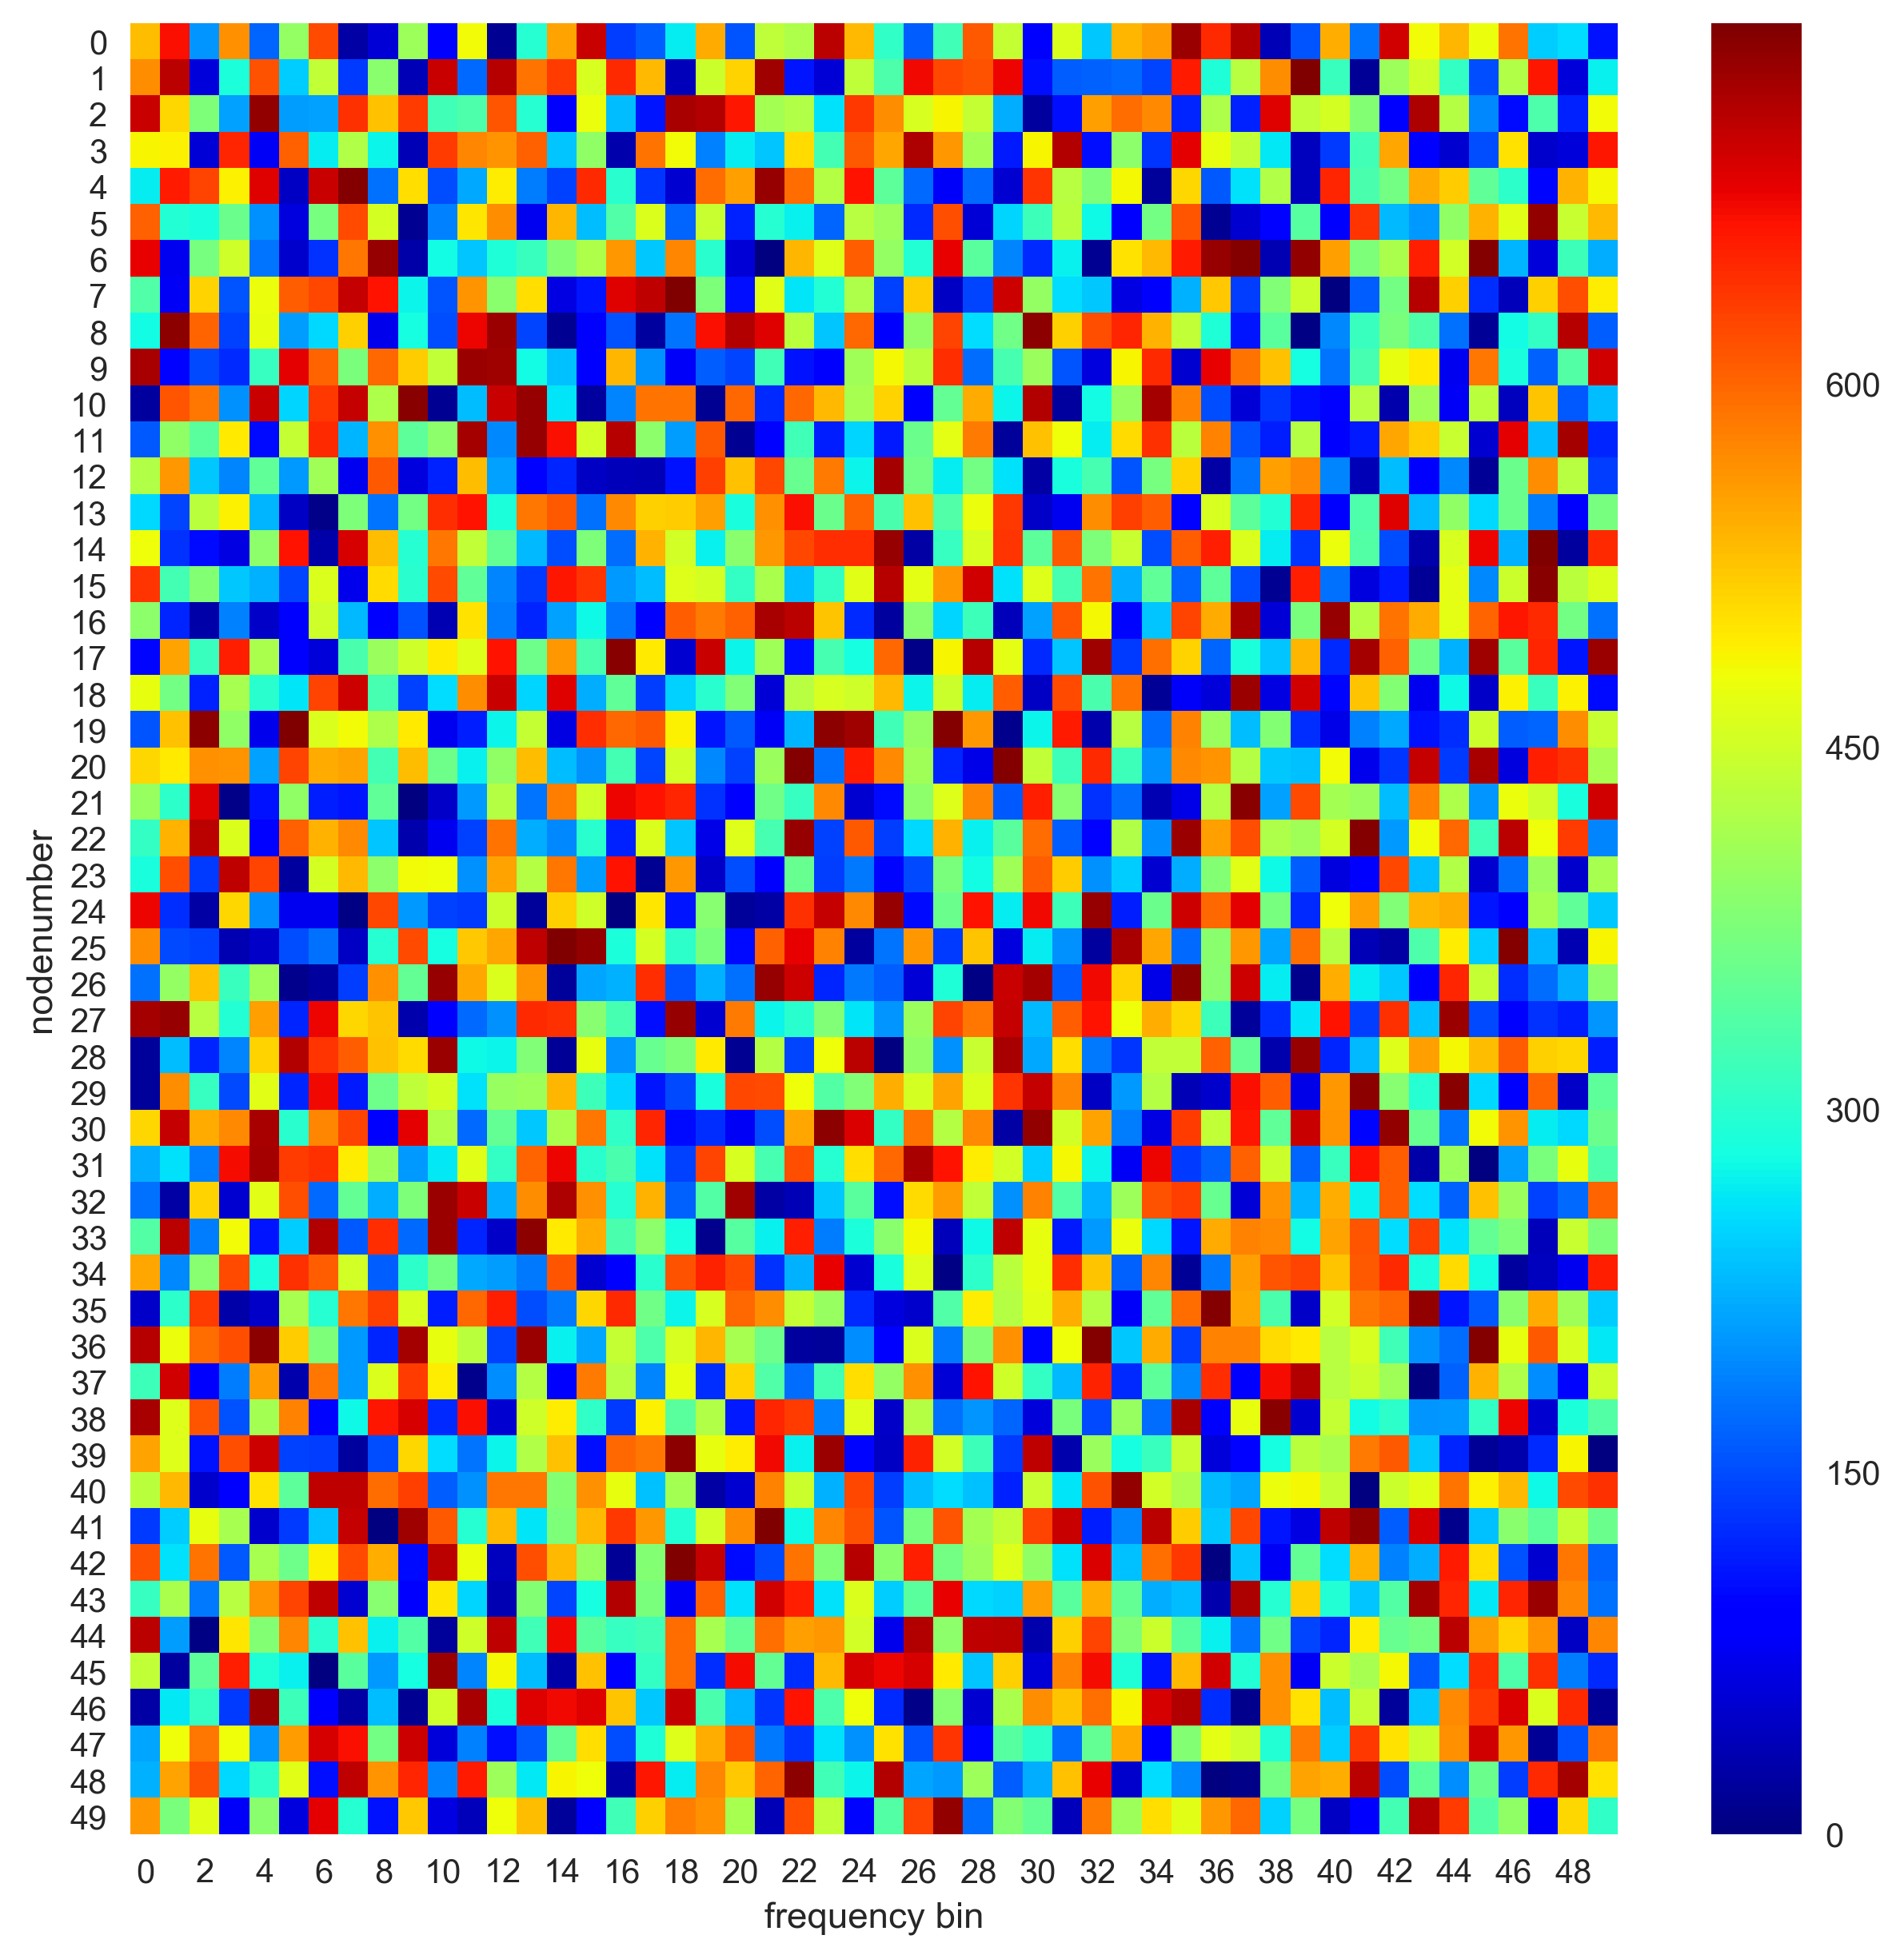
\includegraphics[width=0.85\textwidth]{Pictures/fft_heat.png}
\caption{Exemplary FFT heatmap of magnitude. Random data.}
\label{fft_heat}
\end{figure}

Spectrum plot amplitude range as well as maximum FFT amplitude range are normalized and presented on a logarithmic scale as per formula \ref{eq:FFTnorm}. 

\begin{equation} \label{eq:FFTnorm}
\text{Amp}_{kn} = 20 \cdot \log_{10} \left( \frac{\text{Amp}_{k}}{\text{Amp}_{max}} \right)
\end{equation}

\noindent where $\text{Amp}_{max}$ is the global maximum amplitude of all datasets.

This operation has been performed separately on spectrum plots and peak amplitude plots. For spectrum plots the lower [dB] range is calculated by applying the formula \ref{eq:FFTnorm} to global minimum and global maximum amplitudes, resulting in lower end of the scale of -226.41 dB, rounded down to -230dB. For surface plots, where only peak amplitudes are taken into account, the lower end of the plotting range is set as follows: obtain list of maximum amplitudes from all control surfaces, next take the minimum value from the obtained list and apply the aforementioned formula. The lower limit of the surface amplitude plots is calculated to -62.94 dB, rounded down to -65dB. This ensures that color range on is consistent throughout the spectrum plots and surface plots, with maximum value of 0 on every amplitude plot, corresponding to the maximum amplitude value.

Frequency of maximum amplitude for each node is obtained from the dataset. Moreover an amplitude weighted average frequency is calculated (eq. \ref{eq:AWAF}) to show the dominating frequency range on the given control surfaces. Frequency range presented on these plots is limited slightly above the maximum frequency possible to resolve by the presented approach and the limits are 0Hz and 25000Hz.

\begin{equation} \label{eq:AWAF}
\bar{f} = \frac{\sum_{k=1}^{N} f_{bin_k} \cdot \text{Amp}_k}{\sum_{k=1}^{N} \text{Amp}_{k}}
\end{equation}


%-----------------------------------
%	SUBSECTION
%-----------------------------------
\subsection{Qualitative analysis} \label{fft_res_qual}
Analysis of the spectrum plots of the internal surfaces shows the following phenomena. At lower node numbers -- towards the inlet of the domain, the lower frequencies are dominant in the spectrum, with little or no high frequency constituents. With increasing node numbers -- moving towards the domain outlet, the amplitude of the low frequencies is increasing, whilst the high frequency constituents are also increasing their magnitudes. This pattern is repeated throughout the internal surfaces plots, including the tip internal surface. Moreover, the general observation is, that the magnitudes of given frequency bins, for corresponding node numbers, is increasing along with the distance from the hub. Therefore, the "quietest" region of the flowfield is upstream of the blade and near the hub and the "volume" of the sound increases towards the trailing-edge-to-tip-juncture. One of the most important conclusions appearing from the spectrum plots is, that the flow nearfield sound, although having source in seemingly random flow fluctuations, is not random nor has a characteristic of white noise. The spectrum plots are lacking the information on the node locations, therefore spatial analysis of the plots poses some difficulties. Further analysis is done on internal surface and blade surface plots.

Amplitude weighted average frequency plots reduces the high dimensional FFT dataset to a plot feasible to show in a printed form. Frequency spectrum is averaged and constituents of high amplitude are highlighted on the plot. The averaged frequency is in higher range of c.a. 10kHz on the int-01 surface (Fig. \ref{int-01-awaf}) and up to 15-16kHz on the int-tip surface (Fig. \ref{int-tip-awaf}). These frequencies are represented by a high pitched noise, characteristic to operating jet engines and being one of two main sources of noise of the engine. The plot is consistent with RMS sound pressure and sound intensity plots, suggesting, that the main contributor to the averaged RMS sound pressure is the high frequency noise.

Surface plots of frequencies of maximum FFT amplitude show, that the highest frequency oscillations occur in highly separated regions of the flow: in the wake behind the trailing edge of the blade and in the leading edge-hub juncture induced secondary flow. Surprisingly, the highest frequency fluctuations were captured in tip-to-trailing-edge juncture, which is the region where the largest RMS sound pressure values were noted.

%-----------------------------------
%	SUBSECTION
%-----------------------------------
%\subsection{Quantitative analysis} \label{fft_res_quant}
%Morbi rutrum odio eget arcu adipiscing sodales. Aenean et purus a est pulvinar pellentesque. Cras in elit neque, quis varius elit. Phasellus fringilla, nibh eu tempus 1venenatis, dolor elit posuere quam, quis adipiscing urna leo nec orci. Sed nec nulla auctor odio aliquet consequat. Ut nec nulla in ante ullamcorper aliquam at sed dolor. Phasellus fermentum magna in augue gravida cursus. Cras sed pretium lorem. Pellentesque eget ornare odio. Proin accumsan, massa viverra cursus pharetra, ipsum nisi lobortis velit, a malesuada dolor lorem eu neque.